\documentclass[conference]{IEEEtran}
\IEEEoverridecommandlockouts

\usepackage[T1]{fontenc}
\usepackage[utf8]{inputenc}
\usepackage{cite}
\usepackage{amsmath,amssymb,amsfonts}
\usepackage{graphicx}
\usepackage{booktabs}
\usepackage{tabularx}
\usepackage{array}
\usepackage{xcolor}
\usepackage{placeins}
\usepackage[hidelinks]{hyperref}
\usepackage{xurl}

\graphicspath{{figures/}}
\renewcommand{\tabularxcolumn}[1]{>{\raggedright\arraybackslash}p{#1}}
\newcolumntype{L}[1]{>{\raggedright\arraybackslash}p{#1}}
\newcommand{\ind}{\mathbb{1}}

\begin{document}

\title{Probabilistic Forecasting of Petroleum Imports and Supply-Shortfall Risk in Landlocked Economies}

\author{\IEEEauthorblockN{Imanbek Mashrapov}
\IEEEauthorblockA{Informatics and Engineering Department\\
Ala-Too International University\\
Bishkek, Kyrgyzstan\\
Supervisor: Dr. Remudin Reshid Mekuria}}

\maketitle

\begin{abstract}
Landlocked economies buy almost all of their refined fuel over a few overland routes and from very few suppliers, and they hold small stocks. A decision by one exporter can therefore become a domestic shortage within weeks, as Kyrgyzstan experienced in mid-2026 when AI-95 gasoline ran out at Bishkek filling stations. Existing security-of-supply indices describe this dependence after the fact, and existing trade-forecasting studies mostly predict annual values for single countries, so planners lack a tested, forward-looking measure of supply risk.

This proposal sets out a quantitative, comparative study that will test whether monthly physical imports of refined petroleum, and the probability of a supply shortfall, can be forecast out of sample with calibrated uncertainty using only information public on each forecast date. Simple baselines, gradient-boosted trees and small global neural networks will be compared on a UN Comtrade panel of landlocked economies, with Kyrgyzstan as the detailed case. Preliminary work has produced a validated panel of 44 series from 22 countries (5,549 monthly observations); Kyrgyz gasoline volumes agree with the national energy balance within 3.7\%. Evaluation will use lag-aware rolling origins, proper scoring rules, conformal calibration and formal accuracy tests. The expected contribution is a tested benchmark, a transparent route from customs records to a validated physical target, and a prototype risk monitor.
\end{abstract}

\begin{IEEEkeywords}
petroleum imports, probabilistic forecasting, supply-shortfall risk, landlocked economies, global forecasting models, gradient boosting, conformal prediction, publication lag, Kyrgyzstan.
\end{IEEEkeywords}

% =====================================================================
\section{Introduction}\label{sec:intro}

\subsection{Background of the Study}
Landlocked economies cannot receive fuel through their own seaports. Their refined products cross at least one neighbouring country, and a few refiners or traders can supply nearly all of it. The United Nations lists 32 landlocked developing countries \cite{ohrlls}, yet research on them concentrates on trade costs and transit rather than on forecasting the flows their economies depend on \cite{wto2021}.

Kyrgyzstan illustrates the risk. It uses roughly 1.6 to 2 million tonnes of petroleum products a year, and official statements put Russia's share of supply at about 93\% \cite{economist_stocks,kg24_exempt}. Russia restricted gasoline and diesel exports in 2023 and banned gasoline exports in 2024 and again from October to December 2025 \cite{gta2023,gta2025}. Supplies to Kyrgyzstan were formally exempt, yet in mid-2026 AI-95 gasoline ran out at Bishkek stations, the government banned fuel exports, and stocks fell to two or three weeks of use against a 2.5-month target \cite{kunuz2026,kwan2026}. Customs data captured the event: in August 2026 Kyrgyz gasoline imports in UN Comtrade were 16.9 thousand tonnes (kt), about 39\% of the 2024--2025 monthly average.

UN Comtrade reports monthly imports by country, six-digit Harmonized System (HS) code and partner, with net mass and customs value in separate fields \cite{comtrade}, so physical volume need not be inferred from prices. The data are also released late, revised and sometimes inconsistent \cite{hu2022}. These properties decide what a forecaster could actually have known on any date, and they are part of the problem studied here.

\subsection{Statement of the Problem}
National statistics describe what fuel arrived in the past; they do not say how much is likely to arrive next month, how uncertain that is, or how likely a shortfall is. Supplier-concentration indices describe exposure but are rarely tested as predictors \cite{ang2015}, and the only test found showed concentration to be a weak short-run signal \cite{kwon2026}. Studies that forecast petroleum imports are single-country, mostly annual, mostly in value terms and deterministic \cite{santi2023,qin2026}.

The central research problem is therefore: \emph{to what extent can monthly physical imports of refined petroleum in landlocked economies, and the risk of a supply shortfall, be forecast out of sample with calibrated uncertainty, using only the information available on the forecast date?} Answering it matters because stock policy and emergency purchasing depend on the lower tail of the supply distribution, not on its average.

\subsection{Purpose and Objectives of the Study}
The purpose of the study is to determine whether such forecasts can be made with useful, calibrated accuracy, and under what conditions globally trained deep learning improves on gradient boosting and simple baselines. The specific objectives are to:
\begin{enumerate}
\item build an audited, reproducible monthly panel of refined-fuel imports for landlocked economies, validated against official sources;
\item define a shortfall target that separates supply stress from weak demand;
\item compare baseline, tree-based and global neural models under evaluation that respects publication lags;
\item measure by ablation the value of pooling, supplier structure and shock information;
\item calibrate forecasts and compare shortfall warnings with concentration screening; and
\item deliver a prototype risk monitor.
\end{enumerate}

\subsection{Research Questions and Hypotheses}
The study will answer four research questions, each paired with a working hypothesis that is fixed before modelling and will be tested at the 5\% level with Holm correction \cite{holm1979}. A hypothesis that is not supported is an acceptable, informative outcome. Table~\ref{tab:rqmatch} links each question to its method.

\begin{description}
\item[RQ1] Does training one model across countries improve Kyrgyz forecasts over local models and the seasonal naive benchmark?
\item[H1] Global models reduce Kyrgyz MASE by at least 5\% relative to the best local model at a three-month horizon.
\item[RQ2] Do global neural models outperform gradient boosting in normal and shock periods?
\item[H2] They do not beat LightGBM overall but do beat it in documented shock windows.
\item[RQ3] Do supplier structure and shock information add predictive value beyond a series' own history?
\item[H3] They reduce pinball loss by at least 3\% for high-dependence series.
\item[RQ4] Can calibrated forecasts warn of shortfalls better than concentration screening?
\item[H4] Forecast-based shortfall probability gives higher PR-AUC, and higher recall at a fixed alert budget, than ranking by the Herfindahl--Hirschman index (HHI).
\end{description}

\subsection{Significance of the Study}
The study will contribute a tested benchmark of global deep learning against gradient boosting for monthly physical fuel imports, a transparent route from raw customs records to a validated physical target under real publication lags, and a public-data risk monitor; it does not claim a new neural architecture. It differs from earlier work by joining streams that have been studied separately: trade forecasting at annual or value scale \cite{sellami2024}, backward-looking security-of-supply indices \cite{cohen2011}, and customs-based early warning for a coastal economy \cite{kwon2026}.

The study targets three audiences. Energy ministries, state fuel companies and statistical offices in landlocked economies gain an early, quantified signal for stock planning; fuel importers gain a public estimate of supply risk by product; and forecasting researchers gain evidence on when cross-learning and deep learning help on short, heterogeneous panels, a question on which the literature disagrees \cite{montero2021,yolusever2026}. The study also seeks to change two practices: monitoring supply risk with static indices instead of tested probabilistic forecasts, and evaluating trade forecasts on random splits instead of on data as they were released. The researcher, based in Bishkek, observed the 2026 shortage directly; the study grew from the question of whether public data could have anticipated it.

\subsection{Scope and Delimitations}
The study will forecast monthly imports of a gasoline proxy (HS 271011 and 271012) and of distillates with blends (HS 271019 plus 271020) from January 2015 to the latest available month. Because HS~271019 mixes diesel, kerosene and fuel oil, the second target will be labelled ``distillates,'' never ``diesel.'' Crude oil and liquefied petroleum gas are excluded as targets. Customs records measure imports, not consumption, and the models are not intended to predict political decisions such as export bans.

\subsection{Overview of Methodology and Definition of Terms}
The study will use a quantitative, comparative design in which each research question is answered by changing one component (model class, training scope, information source or output) while data, validation protocol and metrics stay fixed. Forecasts will be made at rolling origins using only data released by each origin, and scored with scale-free errors, proper scoring rules and formal tests. Key terms are used as follows:
\begin{itemize}
\item \emph{Physical imports}: net mass recorded by customs, in tonnes.
\item \emph{Supply shortfall}: a month in which trailing three-month import mass falls below 75\% of its seasonal baseline (Section~\ref{sec:measures}).
\item \emph{Publication lag}: time between the end of a month and the first public release of its record; \emph{as-of evaluation} uses only data released by the forecast origin.
\item \emph{Global model}: one model whose parameters are shared across all series; a \emph{local model} is fitted to one series.
\item \emph{Calibration}: agreement between stated probabilities or interval levels and observed frequencies.
\end{itemize}

Section~\ref{sec:lit} reviews the related literature and identifies the research gap; Section~\ref{sec:method} presents the conceptual framework and methodology. The appendices report preliminary data validation and a small pilot.

% =====================================================================
\section{Review of Related Literature}\label{sec:lit}
The review is organised thematically. It draws on a structured search of OpenAlex, Crossref, Semantic Scholar and arXiv plus citation chasing: 6,526 records reduced to 5,230 unique works, 1,600 were screened and 184 were included after verification against DOI registries. Google Scholar could not be searched systematically, so recall for grey literature is limited.

\subsection{Forecasting Petroleum Imports}
Direct studies are few and single-country. Indonesia's oil and gas imports were forecast with a multilayer perceptron on annual volumes \cite{wanto2019}, SARIMA on monthly values \cite{santi2023} and a gated recurrent unit \cite{saputra2024}; China's import demand with machine-learning regressors \cite{qin2026}; and Nepal's petroleum imports, a landlocked case, econometrically without forecast comparison \cite{pradhan2023}. Three weaknesses recur: values or annual totals instead of monthly physical flows; contemporaneous regressors that are unknown on the forecast date; and single splits with percentage or $R^2$ metrics. One study turned annual data into 200 interpolated points and reported 99\% accuracy \cite{khajoui2024}. Two recent studies come closer, masking inputs by release calendar for oil exports \cite{intarasat2026} or forecasting raw-material trade with a Temporal Fusion Transformer \cite{arrar2025}, but neither produces calibrated forecasts of fuel imports.

\subsection{Energy Security, Concentration and Early Warning}
Energy-security research measures dependence with indices of supplier diversification \cite{cohen2011} and political or transit risk \cite{lecoq2009}; a review of 104 studies found such indices context-specific and hard to compare \cite{ang2015}. They describe exposure after the fact and are rarely tested as predictors. The closest precedent is Kwon and Jeong \cite{kwon2026}, who predicted import-disruption onsets for 5,925 Korean products with walk-forward validation and found that concentration rankings performed below the base rate. Their setting is a maritime economy, all goods and a ranking output; whether their finding holds where one supplier provides over 90\% of fuel is open. Geopolitical shocks, measured by the index of Caldara and Iacoviello \cite{caldara2022}, lower energy import volumes in the short run \cite{lin2025}, and training windows that cross structural breaks can damage fuel forecasts \cite{li2022}, so the 2022--2026 period is a natural stress test.

\subsection{Global Models, Deep Learning and Gradient Boosting}
Global models trained across many series can match or beat local ones \cite{montero2021,hewamalage2022}. This is what makes deep learning feasible here: about 130 Kyrgyz months cannot train a network, but a pooled panel may support a small one. The gain is not guaranteed: pooling reversed on heterogeneous short panels \cite{yolusever2026}, while a multi-country Temporal Fusion Transformer \cite{lim2021} beat regressions for 25 OECD economies \cite{laborda2023}. Recurrent networks \cite{hochreiter1997,cho2014} and N-BEATS \cite{oreshkin2019} are standard neural candidates, but gradient-boosted trees \cite{chen2016,ke2017} dominated the M5 competition \cite{makridakis2022} and remain strong on medium-sized tabular data \cite{grinsztajn2022}. A simple linear model even matched Transformers on larger benchmarks \cite{zeng2023}. The literature therefore supports testing deep learning by regime and treating boosting as the main rival.

\subsection{Probabilistic Forecasting and Real-Time Evaluation}
Probabilistic forecasts should maximise sharpness subject to calibration \cite{gneiting2007cal} and be scored with proper rules such as the continuous ranked probability score \cite{gneiting2007}. Electricity forecasting has a probabilistic benchmark tradition \cite{hong2016}, and conformalised quantile regression offers a model-agnostic way to correct interval coverage \cite{romano2019}. Separately, macroeconomics has shown that accuracy measured on revised data can differ from what was achievable in real time \cite{stark2002,baumeister2011}. Good evaluation practice requires rolling origins \cite{tashman2000}, scale-free errors \cite{hyndman2006} and formal tests \cite{diebold1995,harvey1997}. None of the reviewed fuel-import studies reported calibrated distributions or lag-aware evaluation.

\subsection{Synthesis and Research Gap}\label{sec:gap}
Table~\ref{tab:studies} compares the closest studies and Table~\ref{tab:known} summarises what is and is not yet known.

\begin{table*}[t]
\caption{Comparison of the Principal Related Studies}
\label{tab:studies}
\centering
\footnotesize
\begin{tabularx}{\textwidth}{@{}L{2.9cm}XL{3.6cm}X@{}}
\toprule
Study & Problem and data & Method & Limitation for this study \\
\midrule
Kwon and Jeong \cite{kwon2026} & Disruption warning; Korea, 5,925 products, monthly & Boosting, logistic; walk-forward & Maritime; all goods; ranking only \\
Wanto et al. \cite{wanto2019} & Oil and gas imports; Indonesia, annual & Neural network & Annual; point forecast \\
Santi et al. \cite{santi2023} & Oil and gas import value; Indonesia & SARIMA & Value, not mass; one model \\
Pradhan et al. \cite{pradhan2023} & Petroleum imports; Nepal (landlocked) & Econometric & No forecast comparison \\
Laborda et al. \cite{laborda2023} & GDP; 25 OECD countries & Multi-country TFT & Not trade; supports pooling \\
Cohen et al. \cite{cohen2011} & Supply diversification & HHI index & Not tested as a predictor \\
\bottomrule
\end{tabularx}
\end{table*}

\begin{table}[t]
\caption{What Is Known and Not Yet Known}
\label{tab:known}
\centering
\footnotesize
\begin{tabularx}{\columnwidth}{@{}L{1.7cm}XX@{}}
\toprule
Theme & Established & Not yet known \\
\midrule
Fuel-import forecasting & Single-country point forecasts & Monthly physical forecasts across landlocked economies \\
Global models & Cross-learning helps when series are similar & Whether pooling helps weakly co-moving fuel series \\
Deep learning vs.\ trees & Trees are strong on small tabular data & Whether neural models gain in shock periods \\
Probabilistic forecasting & Proper scoring and conformal calibration & Calibrated distributions for fuel imports \\
Real-time evaluation & Revisions change conclusions in macroeconomics & Lag-aware evaluation of Comtrade forecasts \\
Supply security & Concentration describes exposure & Its predictive value under a dominant supplier \\
\bottomrule
\end{tabularx}
\end{table}

A new country alone is not a gap. The gap appears when the problem's requirements are set against the closest streams: trade forecasting predicts annual or value flows, security-of-supply research measures dependence after the fact, and customs early warning ranks products for a coastal economy. No study was found that tests, for landlocked economies, whether monthly physical fuel imports and shortfalls can be forecast out of sample with calibrated uncertainty under real publication lags, or whether pooling and supplier information help. This is a finding of the stated search, not proof of absence, and the study does not assume the integrated approach is superior; that is the question it will answer.

% =====================================================================
\section{Conceptual Framework and Research Methodology}\label{sec:method}

\subsection{Conceptual Framework}
The framework (Fig.~\ref{fig:framework}) links the information released by a forecast origin, through a forecasting process, to a predictive distribution of future physical imports, from which shortfall probability is derived and evaluated. It draws on the global-model argument \cite{montero2021}, the principle of sharpness subject to calibration \cite{gneiting2007cal} and the real-time-data argument \cite{stark2002}. Its key assumptions are that import dynamics are stable enough within a training window to be learned, that cleaned customs net mass measures physical supply, that a seasonal three-month shortfall is a reasonable proxy for supply stress, and that forecast errors are close enough to exchangeable for conformal calibration. Each will be checked, not assumed. Table~\ref{tab:vars} lists the variables.

\begin{figure*}[t]
\centering
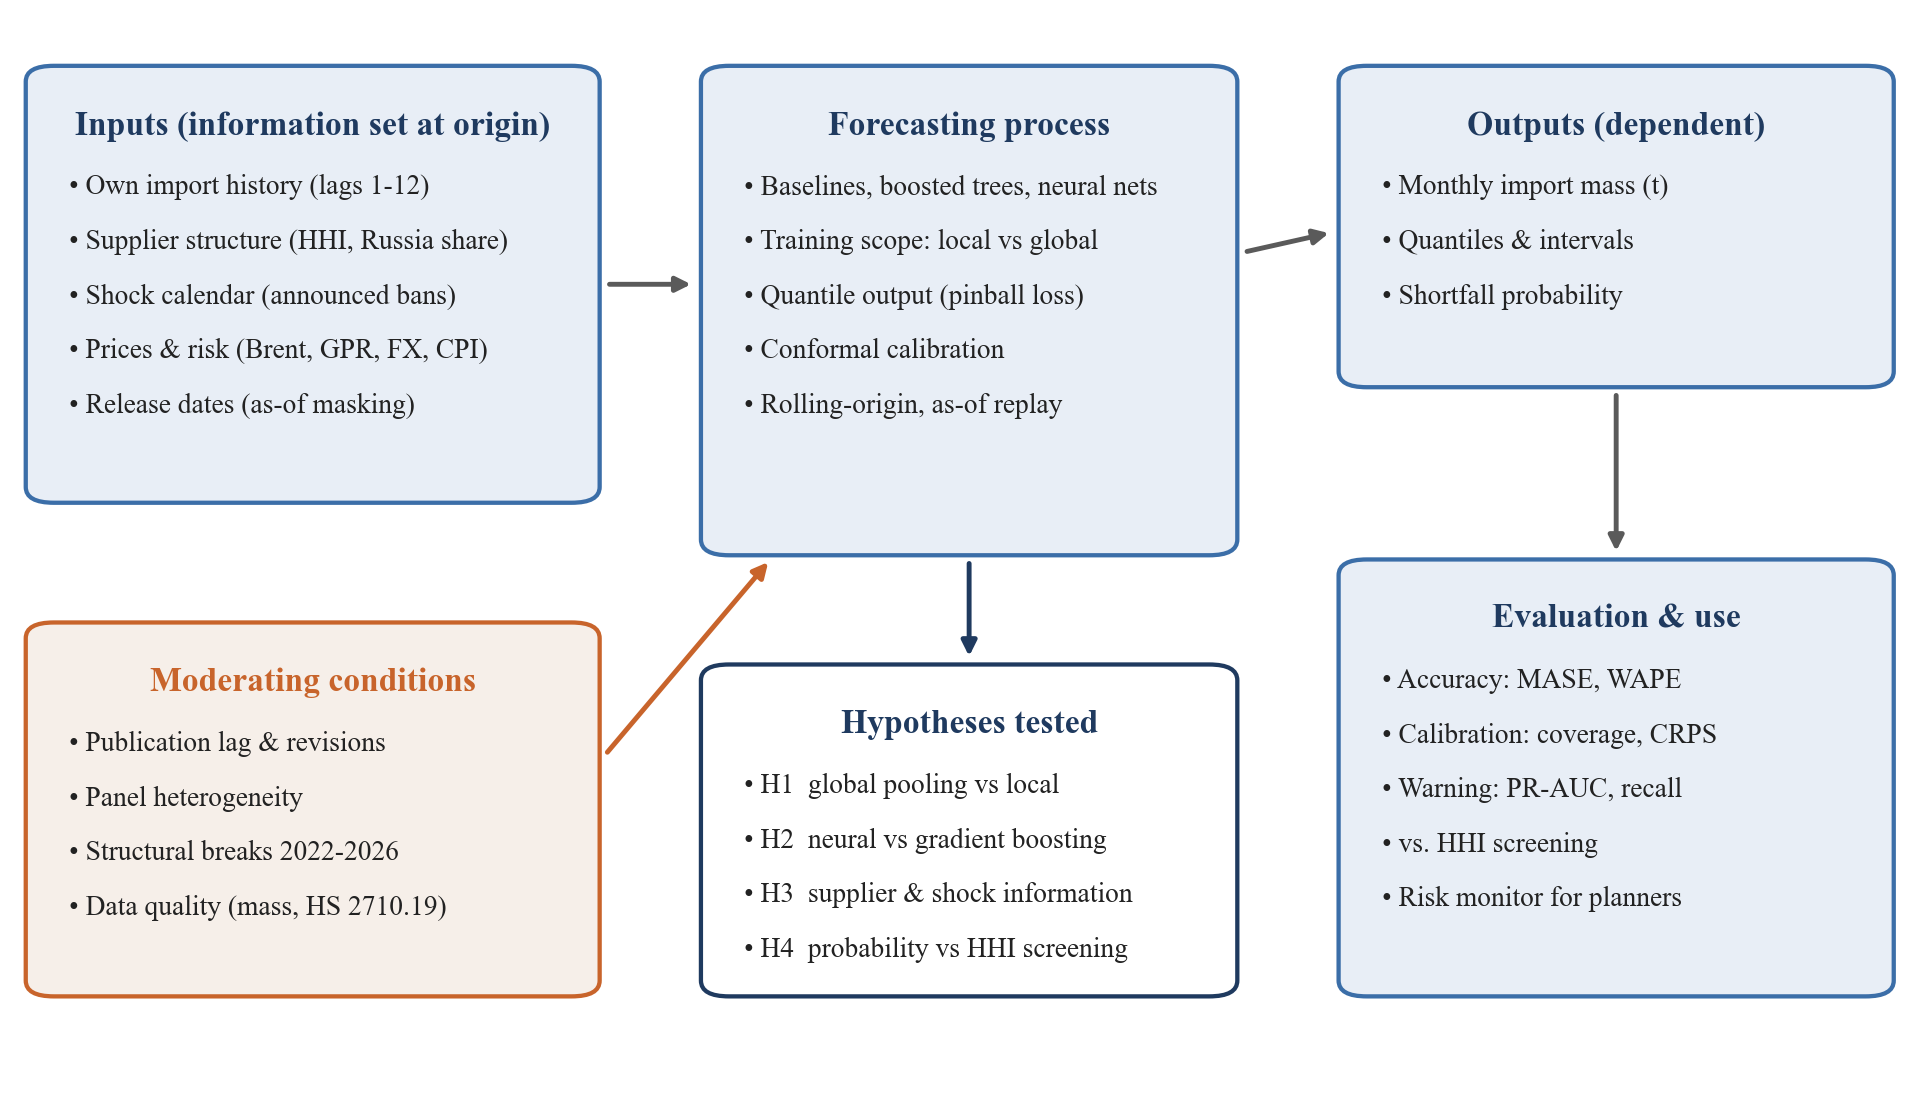
\includegraphics[width=0.82\textwidth]{fig_conceptual.png}
\caption{Conceptual framework of the study.}
\label{fig:framework}
\end{figure*}

\begin{table}[t]
\caption{Variables of the Study}
\label{tab:vars}
\centering
\footnotesize
\begin{tabularx}{\columnwidth}{@{}L{1.6cm}XX@{}}
\toprule
Role & Variable & Measurement \\
\midrule
Dependent & Monthly import mass (gasoline proxy, distillates) & Log tonnes, cleaned net mass \\
Dependent & Shortfall indicator and probability & Eqs.~\eqref{eq:short}--\eqref{eq:risk} \\
Independent (design) & Model class; local or global training & Baseline, boosted tree, neural network \\
Independent (information) & Own history; supplier structure & Lags 1--12; trailing HHI, Russia share \\
Independent (information) & Shocks; prices; risk; macro & Announced bans; Brent; GPR; FX; CPI \\
Moderating & Publication lag, revisions, heterogeneity, breaks & Release dates; vintages; break tests \\
\bottomrule
\end{tabularx}
\end{table}

\subsection{Research Design}
The study will be quantitative, comparative and predictive, based on secondary data. A quantitative design fits because the questions concern measurable accuracy, calibration and detection; a comparative design fits because each question asks whether one modelling choice beats another under identical conditions. The study will not make causal claims: external indicators are candidate predictors, not causes.

\subsection{Data, Sources and Research Setting}
The data will be secondary, quantitative time series (Table~\ref{tab:sources}). The primary records are monthly bilateral customs entries of reporter, HS code, partner, month, net mass and value. Official Kyrgyz statistics will be used for validation, and a hand-coded calendar of export restrictions, each with source and announcement date, will be compiled. The setting is the refined-fuel trade of landlocked economies, extended with European landlocked states that report reliably; the population is every monthly gasoline and distillate import series for these countries in UN Comtrade from 2015. Kyrgyzstan is the detailed case because of its single-supplier dependence, its documented 2026 shortage and its national validation data. No human participants are involved.

\begin{table}[t]
\caption{Data Sources and Their Use}
\label{tab:sources}
\centering
\footnotesize
\begin{tabularx}{\columnwidth}{@{}XL{1.3cm}L{2.4cm}@{}}
\toprule
Source & Frequency & Use \\
\midrule
UN Comtrade API \cite{comtrade} & Monthly & Targets, suppliers, release dates \\
Russia as reporter (mirror data) & Monthly & Cross-check of Kyrgyz imports \\
NSC energy balance and reports \cite{nsc_balance} & Annual, monthly & Mass and value checks; vintages \\
Brent price \cite{eia_brent}; GPR \cite{caldara2022} & Daily, monthly & External conditions \\
Exchange rates, CPI, World Bank indicators \cite{wdi} & Monthly, annual & External conditions; scale \\
Export restrictions \cite{gta2023,gta2025} & Event & Shock calendar \\
\bottomrule
\end{tabularx}
\end{table}

\subsection{Data Collection Procedure and Sampling}
Data will be collected by a Python pipeline that queries the Comtrade API with credentials kept in environment variables, stores each raw response with its retrieval date and hash, and writes versioned datasets. This instrument already exists: it holds 878 validated responses and passes 24 automated tests. A second snapshot will be taken before modelling so that revisions can be measured.

No random sample will be drawn. Series will be selected purposively by rules fixed before modelling (Table~\ref{tab:tiers}). In preliminary work these rules gave an evaluation set of 22 series from 13 countries (3,021 monthly observations) and a training pool of 44 series from 22 countries (5,549 observations); Fig.~\ref{fig:coverage} shows coverage. Kyrgyzstan is the only Central Asian country in Tier~1.

\begin{table}[t]
\caption{Series Selection Criteria by Tier}
\label{tab:tiers}
\centering
\footnotesize
\begin{tabularx}{\columnwidth}{@{}L{0.6cm}XL{1.6cm}@{}}
\toprule
Tier & Criteria & Use \\
\midrule
1 & $\geq$120 observed months; $\geq$85\% coverage; no gap over six months; data to mid-2025 or later; $\geq$84 supplier months; median $\geq$100\,t; exports below half of imports & Evaluation and training \\
2 & $\geq$84 observed months and $\geq$84 supplier months & Training only \\
3 & Sparse or unusable reporting & Descriptive only \\
\bottomrule
\end{tabularx}
\end{table}

\begin{figure}[t]
\centering
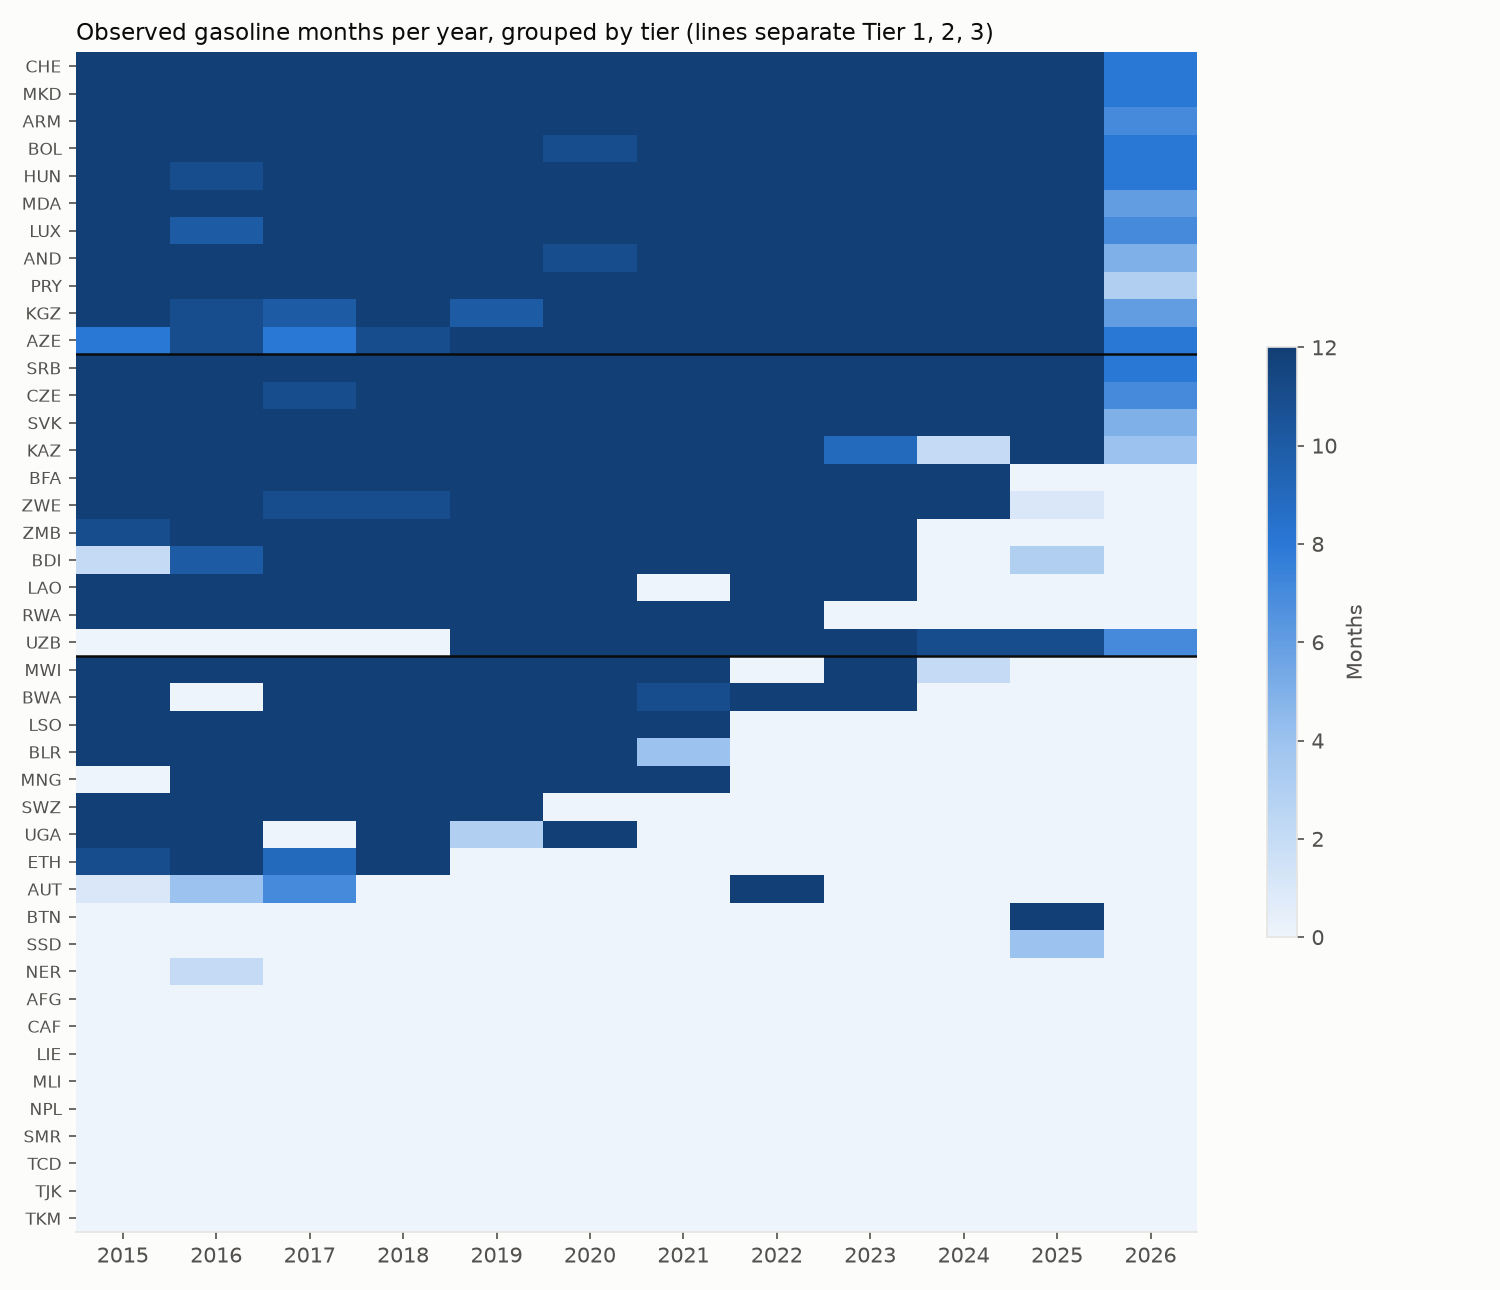
\includegraphics[width=\columnwidth]{fig09_coverage_heatmap.png}
\caption{Observed gasoline months per year by reporting country. Lines separate Tiers 1, 2 and 3.}
\label{fig:coverage}
\end{figure}

\subsection{Data Preparation}
Monthly totals will be rebuilt from partner rows, because the aggregate ``World'' row can be zero while partner rows contain trade. Masses will be accepted only in kilograms, with physically plausible implied densities, and unit values will be checked against a Brent-deflated rolling median; implausible masses will be removed while the original record is kept. Outliers will be flagged but kept, because shocks are the object of study. Missing months will never be filled with zeros and targets will never be interpolated; missing months will be excluded from training loss and scoring.

\subsection{Key Measures}\label{sec:measures}
Supplier concentration will be measured with the HHI, where $s_{ijt}$ is the share of partner $j$ in the import mass of series $i$ in month $t$, pooled over a trailing twelve months:
\begin{equation}
\mathrm{HHI}_{it}=\sum_{j} s_{ijt}^{2}. \label{eq:hhi}
\end{equation}
With $Q_{it}$ the trailing three-month import mass and $B_{it}$ the mean of the same calendar months in the previous three years, a shortfall month is
\begin{equation}
S_{it}=\ind\!\left[\,Q_{it}/B_{it}<0.75\,\right], \label{eq:short}
\end{equation}
with thresholds of 0.70 and 0.80 as sensitivity checks. Shortfall risk will be derived from each model's forecast distribution, given the information set of data released by origin $\tau$, where $r_{it}$ is the release date of observation $t$:
\begin{equation}
\hat p_{i,\tau+h}=\Pr\!\left(\frac{Q_{i,\tau+h}}{B_{i,\tau+h}}<0.75 \,\middle|\, \{x_{it}: r_{it}\le\tau\}\right). \label{eq:risk}
\end{equation}

\subsection{Models and Data Analysis}
\emph{Models.} Models will be added in order of complexity so that each component's benefit can be measured: naive, seasonal naive and twelve-month mean (lower bounds); ETS and SARIMA (local references); random forest \cite{breiman2001}; LightGBM and XGBoost (main rivals); and small global GRU, TCN and N-BEATS networks and a compact Temporal Fusion Transformer, retained only if validation supports it. Neural capacity will stay small (16--64 hidden units, a country embedding, dropout). Learned models will output quantiles by minimising pinball loss, and conformalised quantile regression \cite{romano2019} will adjust intervals on a later calibration window.

\emph{Validation.} Evaluation will use expanding rolling origins from January 2023, with horizons of one, three and six months plus the next-three-month total. At each origin only data released by that date will be visible; where a release date is missing, the reporter's median lag will be applied. Random splits will not be used. Tuning will use only past data, and settings will be frozen before a final test block run once. Leave-one-country-out training will test transfer.

\emph{Metrics and tests.} MASE \cite{hyndman2006} will be the primary point metric because it is comparable across countries; with seasonal period $m=12$,
\begin{equation}
\mathrm{MASE}=\frac{\frac{1}{n}\sum_{t}|y_t-\hat y_t|}{\frac{1}{T-m}\sum_{t=m+1}^{T}|y_t-y_{t-m}|}. \label{eq:mase}
\end{equation}
Quantiles will be scored with pinball loss and an approximate CRPS, intervals by coverage and width at 80\% and 95\%, and shortfall warnings by PR-AUC, Brier score \cite{brier1950} and recall at a fixed alert budget, which suit rare events \cite{saito2015}. Model differences will be tested with the corrected Diebold--Mariano test \cite{harvey1997} with Holm correction, and effect sizes with bootstrap intervals will always be reported because tests have low power on short samples. An ablation will remove one information source at a time (pooling, supplier features, shock calendar, external indicators, pre-2022 data, conformal step), and SHAP values \cite{lundberg2017} will help explain LightGBM forecasts. Table~\ref{tab:rqmatch} matches each research question to its method.

\begin{table*}[t]
\caption{Matching of Research Questions to Methods and Evaluation}
\label{tab:rqmatch}
\centering
\footnotesize
\begin{tabularx}{\textwidth}{@{}L{1.4cm}XL{4cm}X@{}}
\toprule
RQ / H & Manipulated component & Comparison & Evaluation \\
\midrule
RQ1 / H1 & Global vs.\ local training & Best local model, seasonal naive & MASE at $h=3$; HLN test \\
RQ2 / H2 & Neural (GRU, TCN, N-BEATS, TFT) vs.\ boosted trees & LightGBM & MASE and pinball loss by normal and shock windows \\
RQ3 / H3 & Supplier and shock features added or removed & Own-history model & Pinball loss, high-dependence series \\
RQ4 / H4 & Calibrated shortfall probability & HHI ranking & PR-AUC, recall at alert budget, calibration \\
\bottomrule
\end{tabularx}
\end{table*}

\subsection{Flow of Research Activities and Data Recording}
Fig.~\ref{fig:flow} and Table~\ref{tab:plan} show the planned stages. Every raw response, dataset and forecast will be stored with its version, date and input snapshot, all figures will be regenerated from scripts, and a decision log will record each change to rules or settings.

\begin{figure*}[t]
\centering
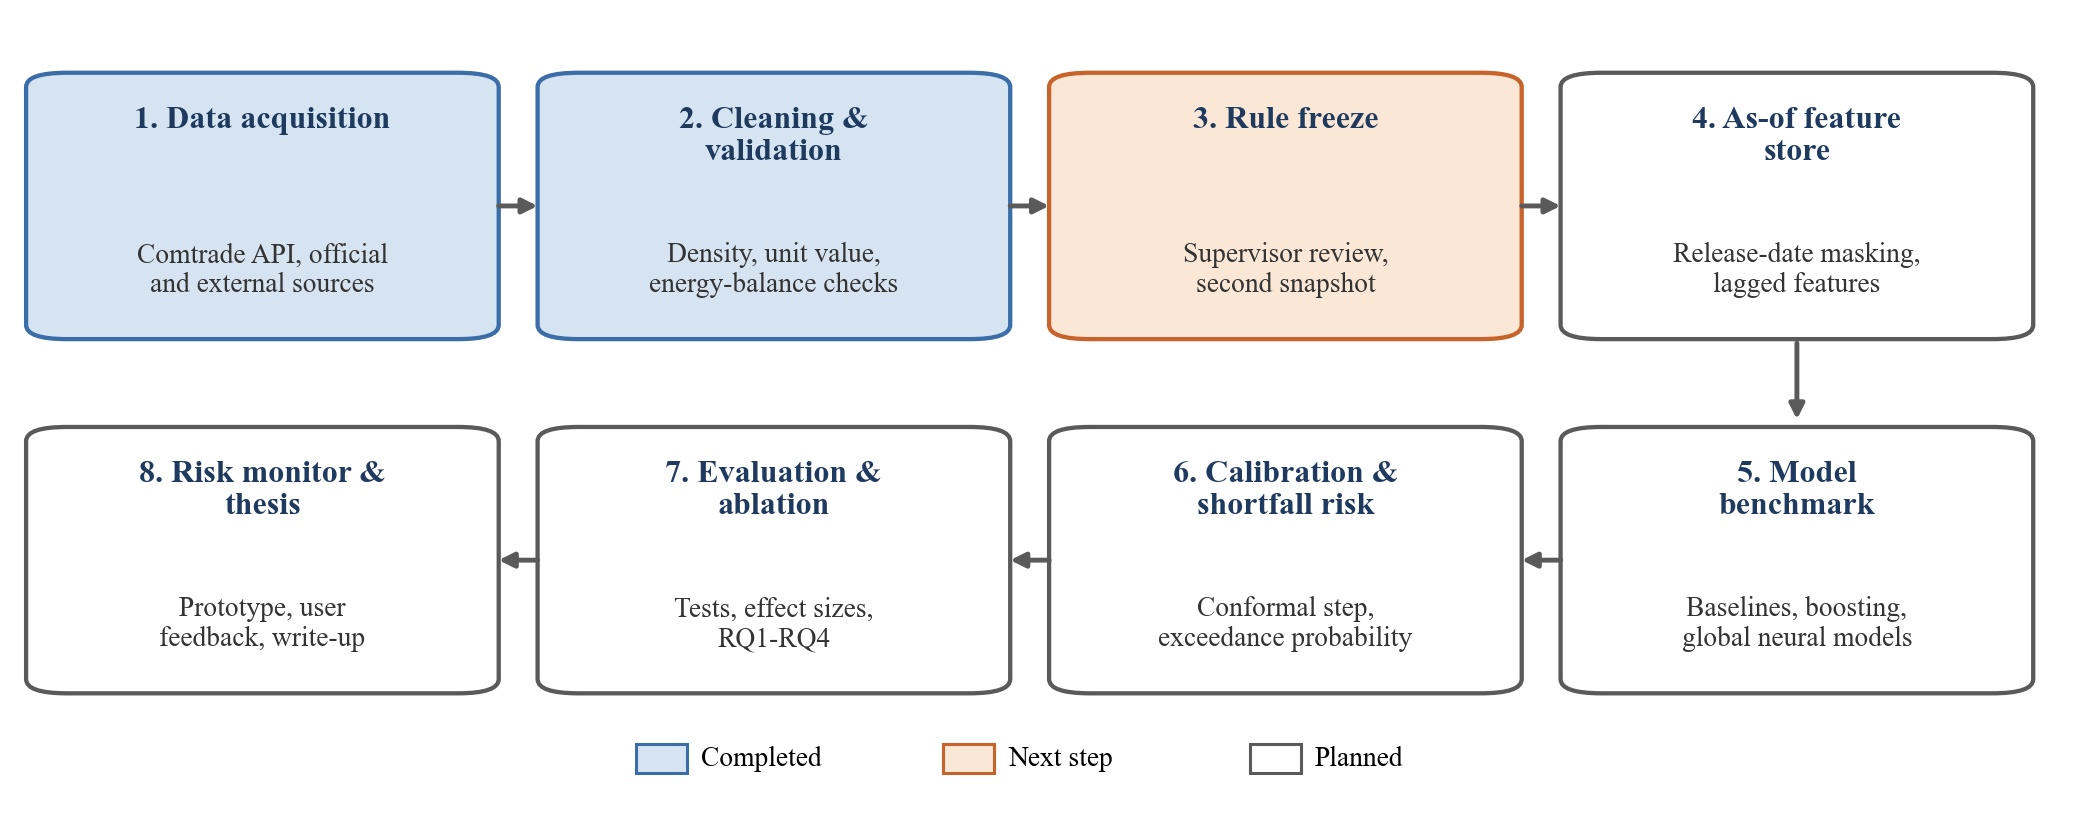
\includegraphics[width=0.9\textwidth]{fig_flow.png}
\caption{Flow of research activities. Shaded stages are complete; the orange stage is next.}
\label{fig:flow}
\end{figure*}

\begin{table}[t]
\caption{Research Stages, Outputs and Indicative Schedule}
\label{tab:plan}
\centering
\footnotesize
\begin{tabularx}{\columnwidth}{@{}XL{2.6cm}L{1.3cm}@{}}
\toprule
Stage & Output & Timing \\
\midrule
1--2. Data acquisition and validation & Validated dataset v1.0 & Completed \\
3. Rule review and second snapshot & Frozen rules; revision log & Month 1 \\
4. As-of feature store & Feature tables by origin & Months 1--2 \\
5--6. Model benchmark and calibration & Forecast archive; calibrated quantiles & Months 2--3 \\
7. Evaluation, ablation, robustness & Tests of H1--H4 & Month 4 \\
8. Risk monitor and thesis & Prototype; final thesis & Months 5--6 \\
\bottomrule
\end{tabularx}
\end{table}

\subsection{Reliability and Validity}
Reliability will rest on versioned snapshots, frozen rules, scripted analysis, at least five random seeds and matched tuning budgets. The main threat to internal validity is information leakage, which will be controlled by as-of replay, by fitting all preprocessing on past data only, and by using a shock only after it was announced. Construct validity has been checked in preliminary work (Appendix~\ref{app:validation}): Kyrgyz gasoline mass agrees with the national energy balance within a mean absolute 3.7\% from 2018. Because 2016--2017 mirror data disagree sharply and post-2025 records appear to be first releases, results will be reported with and without 2015--2017 and evaluated on first-release data. External validity will be examined by leave-one-country-out tests and sensitivity checks on thresholds, lags, COVID-19 months and structural breaks \cite{bai2003}; no claim will rest on a single shock.

\subsection{Ethical Considerations}
All data are public, aggregate and non-personal, and will be used within their providers' terms; API keys will never be stored in code. The work supports supply planning and gives no guidance on evading trade restrictions. Any practitioner review of the prototype will be voluntary and anonymous. Negative results will be reported as prominently as positive ones, all sources will be cited, and AI assistance will be disclosed in line with faculty rules.

\FloatBarrier
% =====================================================================
\appendices

\section{Preliminary Data Validation Results}\label{app:validation}
This appendix reports work already executed on the data snapshot of 2 November 2026 (dataset version 1.0.0). It is descriptive; no forecasting model was fitted to the final datasets. Table~\ref{tab:validation} summarises the checks, and Fig.~\ref{fig:kgz} shows the Kyrgyz series.

\begin{table}[t]
\caption{Validation of the Kyrgyz Comtrade Series}
\label{tab:validation}
\centering
\footnotesize
\begin{tabularx}{\columnwidth}{@{}XL{3.2cm}@{}}
\toprule
Check & Result \\
\midrule
Gasoline mass vs.\ energy balance & 3.7\% mean abs.\ difference from 2018 \\
Gasoline value vs.\ NSC table & Within 5\% in 2022--2024 \\
2025 gasoline value vs.\ NSC & Ratio 0.78 (first release suspected) \\
Gasoline exports vs.\ balance (2024) & 77.6 vs.\ 76.4 kt \\
Partner-row sum vs.\ World row & No month over 5\% in value \\
Russian mirror, 2018 and 2021 & Ratio 0.93--1.02 \\
Russian mirror, 2016--2017 & Ratio 0.33--0.37 (cause unknown) \\
Usable Kyrgyz months per product & 133 of 140 \\
\bottomrule
\end{tabularx}
\end{table}

\begin{figure*}[t]
\centering
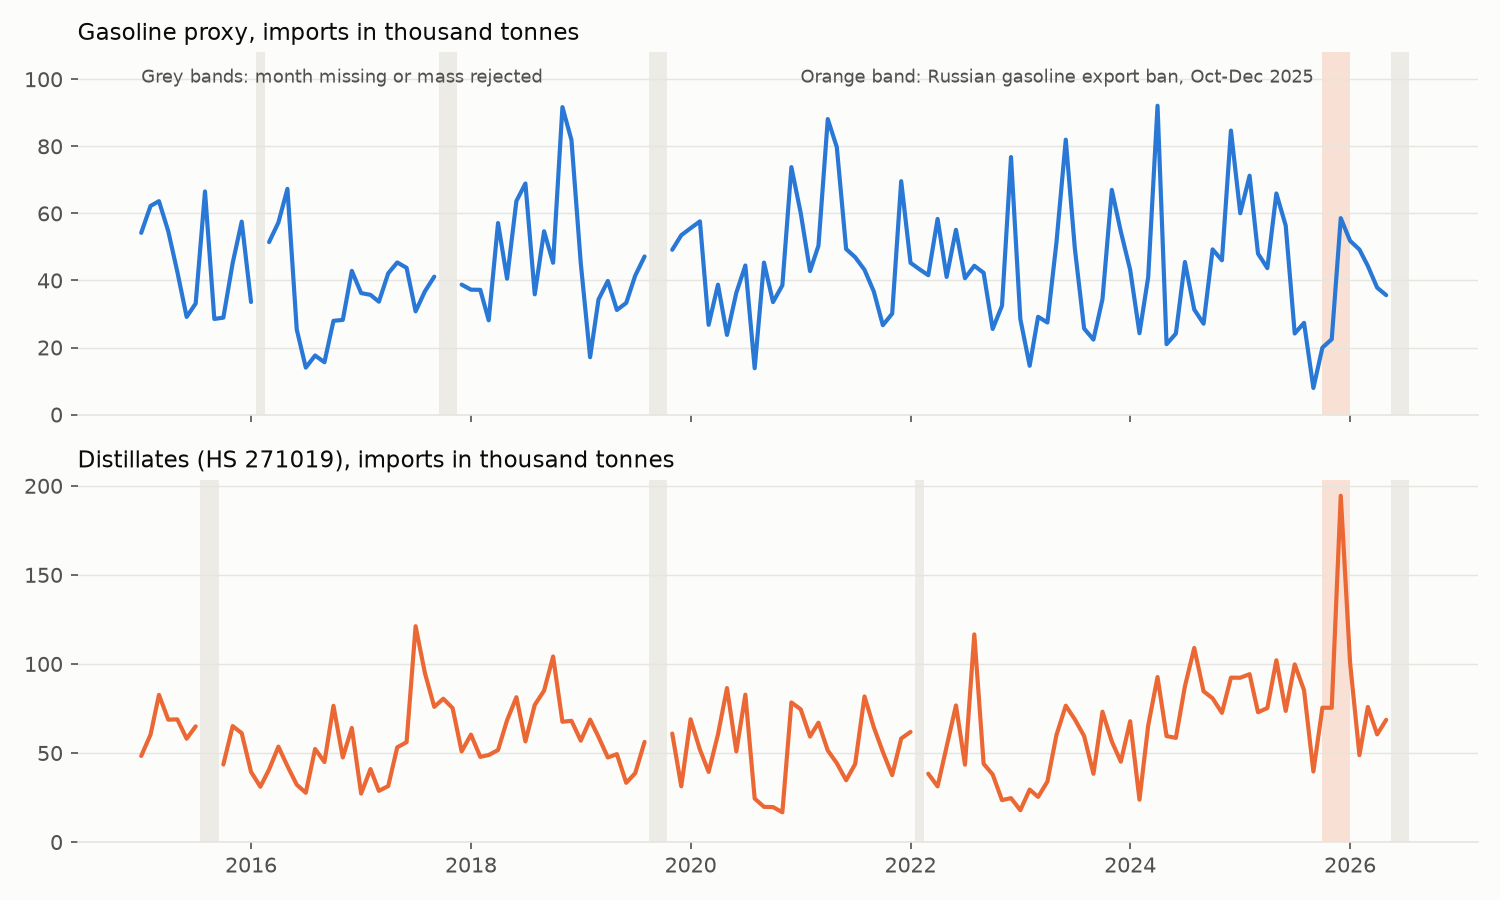
\includegraphics[width=0.85\textwidth]{fig01_kyrgyz_monthly_imports.png}
\caption{Kyrgyz monthly imports, January 2015 to August 2026, in thousand tonnes. Grey bands mark missing or rejected months; nothing is interpolated.}
\label{fig:kgz}
\end{figure*}

Exploratory analysis found that Kyrgyz gasoline imports vary significantly by calendar month (Kruskal--Wallis $p<0.001$), highest in December and lowest in September, while distillates show no clear seasonal pattern ($p=0.42$). Co-movement between countries is weak: the median pairwise correlation of year-on-year gasoline changes is 0.04. Kyrgyz gasoline has a median trailing-twelve-month HHI of 0.89 (Fig.~\ref{fig:hhi}), which leaves little variation for concentration to explain and is a direct difficulty for H4. Net import dependency in 2024 was 0.77 for gasoline and 0.86 for diesel. The clean data give 11 gasoline and 7 distillate shortfall episodes among 112 evaluable months under \eqref{eq:short}.

\begin{figure}[t]
\centering
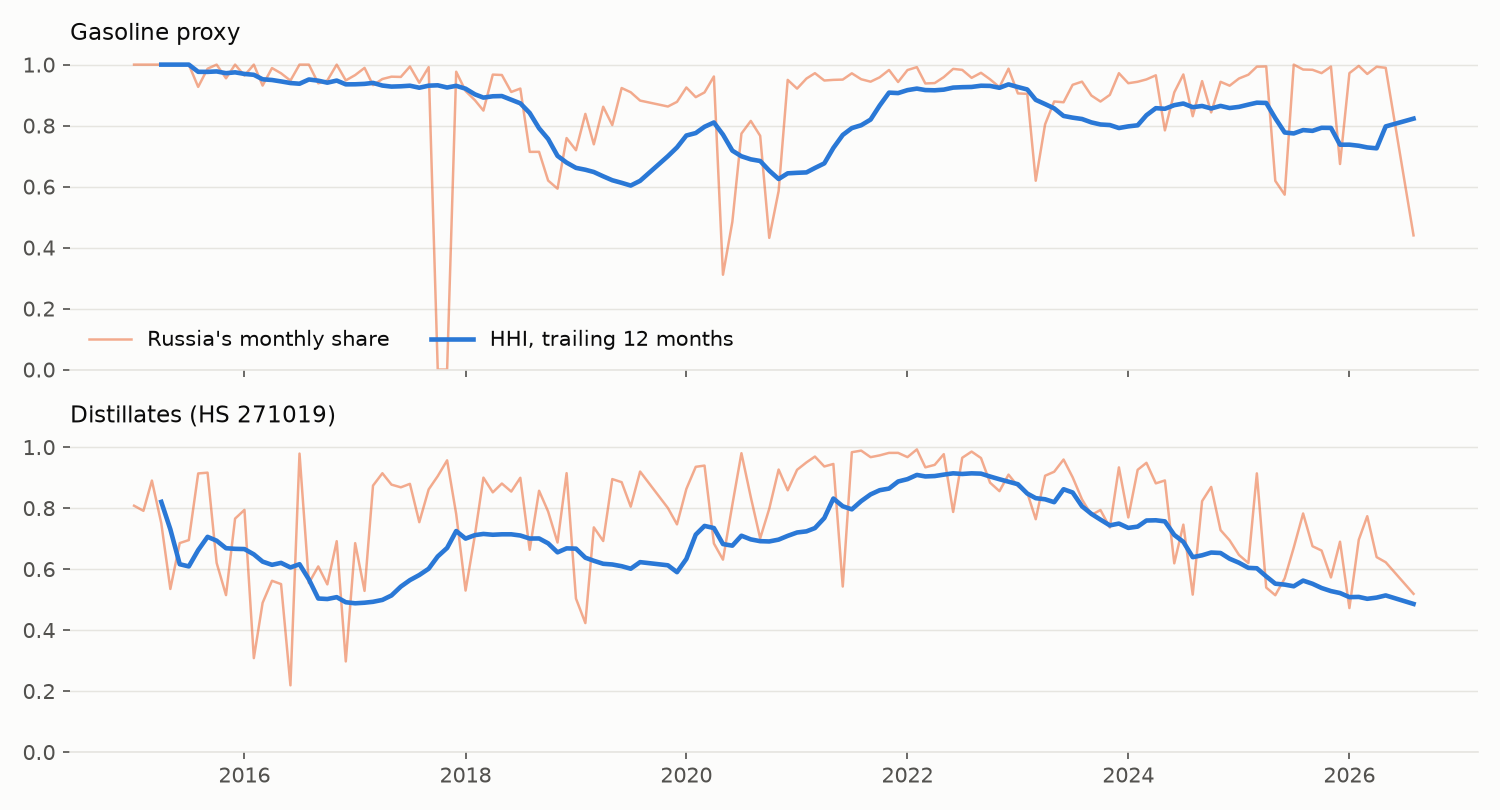
\includegraphics[width=\columnwidth]{fig08_kyrgyz_supplier_concentration.png}
\caption{Kyrgyz supplier concentration (trailing HHI) and Russia's monthly share.}
\label{fig:hhi}
\end{figure}

\section{Untuned Pilot Forecast}\label{app:pilot}
A small, deliberately untuned pilot was run only to check that the design can be executed end to end. It used an earlier 43-series panel with World-row totals, without as-of replay, and test targets from September 2024 to August 2026 (Table~\ref{tab:pilot}). About 22 Kyrgyz test months are too few to rank models, and no significance test was run; the results are indicative only and are not findings of the study.

\begin{table}[t]
\caption{Untuned Pilot: Kyrgyz Gasoline WAPE (\%). Lower Is Better}
\label{tab:pilot}
\centering
\footnotesize
\begin{tabular}{@{}lccc@{}}
\toprule
Model & $h=1$ & $h=3$ & Next 3 months \\
\midrule
Seasonal naive & 49.6 & 49.6 & 29.2 \\
12-month mean & 38.9 & 39.5 & 28.4 \\
LightGBM, local & 30.4 & 32.0 & 20.7 \\
LightGBM, global & 30.6 & 34.8 & 23.6 \\
GRU, global & 33.5 & 42.9 & 28.5 \\
\bottomrule
\end{tabular}
\end{table}

The next-three-month error fell from about 28\% for the twelve-month mean to about 21\% for local LightGBM, which suggests there is signal to model. For August 2026 the median forecast was 38.1\,kt with a lower bound of 20.5\,kt, while the actual value was 16.9\,kt: autoregressive features alone did not anticipate the shock, and nominal 80\% intervals covered only 62--75\% of Kyrgyz outcomes. These observations motivate the calibration step and the supplier and shock features tested under H3 and H4.

\FloatBarrier
\bibliographystyle{IEEEtran}
\bibliography{references}

\end{document}
